\chapter{Neuroevolution}\label{chapter:neuroevolution}
This chapter provides the reader with insight into neuroevolution with primary focus on neuroevolution of augmenting topologies (NEAT), a derivative of a Topology and Weight Evolving Artificial Neural Network (TWEANN). An introduction to neuroevolution is given in Section \ref{sec:ne_introduction}. The historical background is explored in Section \ref{sec:ne_historical_background}. Neural architecture search is discussed in Section \ref{sec:ne_nas}. Section \ref{sec:nn_nutshell} provides the reader with the basic concepts of neural networks which is followed by the main topic, NEAT, in Section \ref{sec:ne_neat}.

\section{Introduction}\label{sec:ne_introduction}
Neuroevolution refers to the optimization of artificial neural networks (ANNs) using evolutionary algorithms (\cite{risi2015neuroevolution}). Unlike traditional gradient-based methods which typically rely on backpropagation and gradient descent to train network weights, neuroevolution employs evolutionary processes inspired by Darwinian evolution to evolve both the architecture and parameters of the neural the network. This approach enables capabilities that traditional gradient-based approaches lack, that is, learning neural network topology configurations such as activation functions, hyperparameters, and architectures (\cite{stanley2019designing}). A more detailed comparison with conventional neural network training techniques in provided in Section \ref{sec:nn_nutshell}.

\parbreak\noindent At its core, neuroevolution treats the design and training of neural networks as an optimization problem in a high-dimensional space. With reference to the evolutionary principles discussed in Chapter \ref{chapter_ea}, candidate solutions are represented as encoded genetic structures, such as chromosomes or vectors, and are subjected to evolutionary processes like mutation, crossover, and selection. Over successive generations, these processes explore the artificial network's configuration, refining the architectures and weight setting in an attempt to optimize the given task at hand (\cite{risi2015neuroevolution}). Neuroevolution offers unique advantages over traditional neural network training methods. For instance, neural networks are traditionally designed manually through trial and error which can become frustrating and cumbersome - neuroevolution does this autonomously.

\section{Historical Background}\label{sec:ne_historical_background}
The development of neuroevolution can be traced back to the early exploration of both neural networks and evolutionary algorithms as separate disciplines in the mid-20th century (\cite{stanley2002evolving}). Evolutionary algorithms, inspired by Darwinian principles of natural selection, were initially applied to optimization problems in the engineering and biology realm. Around the same time, neural networks emerged as a powerful framework to mimic and model cognitive processes (\cite{stanley2002evolving}). By the late 1980s and early 1990s, researchers began to combine these fields, laying the groundwork for what is now known as neuroevolution (\cite{stanley2002evolving}).

\parbreak\noindent By the 1990s, studies demonstrated that the complexity of an artificial network's topology affects the speed of evaluating the network and its learning rate, and that evolving structures saves times wasted by humans trying to decide what the topology of a neural network should look like for a given problem (\cite{stanley2002evolving}). Recurrent Neural Networks (RNNs), a type of artificial neural network designed to recognize sequential patterns by retaining a "memory" of previous inputs through hidden feedback loops, were further advanced by Peter J. Angeline, Gregory M. Saunders, and Jordan Pollack. Their work in evolving RNNs demonstrated neuroevolution's potential for uncovering complex temporal structures (\cite{angeline1994evolutionary}). Kenneth o. Stanley's introduction of Neuroevolution of Augmenting Topologies (NEAT) algorithm in 2002, an extension of TWEANN, marked a significant milestone, showcasing the ability to evolve both a neural network's topology and weights simultaneously (\cite{stanley2002evolving}). NEAT's innovative approach to preserve diversity through speciation and historical marker tracking addressed key challenges that neuroevolution faced such as premature convergence and the difficulty in evolving candidate solutions that represented complex structures (\cite{stanley2002evolving}).

\parbreak\noindent The 2000s and 2010s witnessed the rise of more sophisticated algorithms, such as HyperNEAT, which extended NEAT to large-scale, high-dimensions problems by evolving networks that exploit geometric regularities (\cite{stanley2009hypercube}). In parallel to this, evolutionary strategies (ES) gained traction in optimizating continuous network parameters, particularly in reinforcement learning. By integrating neuroevolution with reinforcement learning, researchers unlocked new capabilities for solving optimization problems that require agents to adapt dynamically in changing environments (\cite{igel2003neuroevolution}).

\parbreak\noindent Today, neuroevolution continues to grow, benefiting from advancements in distributed systems (and thereby computational power), and hybrid approaches that combine evolutionary algorithms with gradient-based methods (\cite{asseman2021accelerating}). The historical progression of neuroevolution reflects a shift from parameter optimization to the co-evolution of architectures and topology parameters, establishing its role as a unique and powerful technique in the artificial intelligence realm.

\section{Neural Networks in a Nutshell}\label{sec:nn_nutshell}
Neural networks form the backbone of modern artificial intelligence (AI), offering a framework to learn complex relationships from a set of data. They are inspired by the biologicinamely, the cell body, dendrites, and axon as shown in Figure \ref{fig:ne_biological_neuron}.

\parbreak
\begin{figure}[H] % Use [H] to suppress floating and place the figure/table exactly where it is specified in the text
	\centering % Horizontally center the figure on the page
	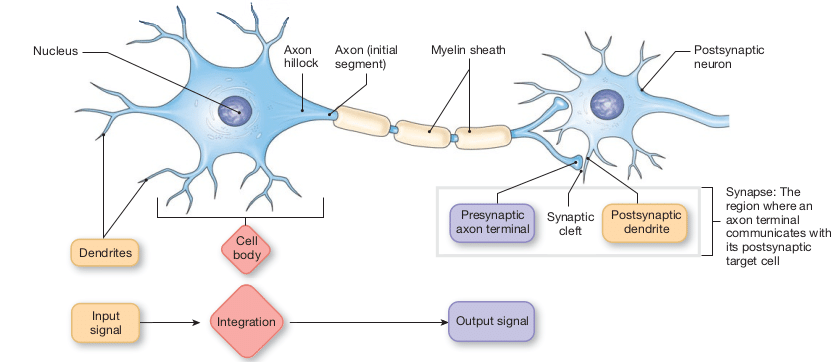
\includegraphics[width=\textwidth]{Figures/chapter_ne/biological_neuron.png} % Include the figure image
	\caption{Simplified illustration of neuron anatomy (\cite{neuron_model})}
	\label{fig:ne_biological_neuron} % Unique label used for referencing the figure in-text
\end{figure}

\parbreak\noindent These neurons communicate through electrical signals by mean of impulses (aka signal) in the cell wall. The impulses are mediated through the junctions called \textit{synapses} which are located on branches of the cell known as \textit{dendrites} (\cite{gurney2018introduction}). The neurons in turn are interconnected with many other neurons which are sending and receiving a multitude of incoming signals simultaneously. The signals are summed together in some way, but unlike in artificial models, where this is often a simple amplitude-based threshold, biological neurons rely heavily on the frequency of incoming spikes to determine firing. If the combined input (weighted by timing and firing rate) exceeds the neuron's threshold, it generates a voltage response (and thereby \textit{"fire"}) (\cite{gurney2018introduction}). The \text{synapse} is categorized as either being an excitory synapse which encourages the subsequent neuron from firing, or it can be an inhibitory synapse which discourages the subsequent neuron from firing (\cite{bishop1994neural}). Whether the \textit{synapse} is excitory or inhibitory is dictated by its strength (or weight). Provided that the neuron is \textit{"fired"}, a signal is sent to other neurons via the \textit{axon} and serve as input to the subsequent neuron (\cite{gurney2018introduction}).

\subsubsection{The Artificial Neuron}
\noindent At their core, neural networks are computational systems that consist of interconnected nodes that mimic the biological neuron seen in Figure \ref{fig:ne_biological_neuron}. Akin to the biological neural system, an artificial neuron is depicted in Figure \ref{fig:ne_artificial_neuron}. 

\parbreak
\begin{figure}[H] % Use [H] to suppress floating and place the figure/table exactly where it is specified in the text
	\centering % Horizontally center the figure on the page
	\includesvg[width=\textwidth]{Figures/chapter_ne/ne_artificial_neuron.svg} % Include the figure image
	\caption{Perceptron (Artificial Neuron) model (adapted from \cite{russell2016artificial})}
	\label{fig:ne_artificial_neuron} % Unique label used for referencing the figure in-text
\end{figure}

\parbreak\noindent The weighted sum (transfer function) depicted in Figure \ref{fig:ne_artificial_neuron} can be represented mathematically as follows (adapted from \cite{suzuki2011artificial}):
\begin{ceqn}
    \begin{equation}\label{alg:osum}
        O_{transfer\_function} = \sum_{i = 1}^{n}w_{ij}x_{i}+b
    \end{equation}
\end{ceqn}

\noindent where:
\begin{itemize}
    \item $x_{i}$ is the input signal
    \item $w_{ij}$ is the weight of the neuron
    \item $b$ is the bias
    \item $O_{transfer\_function}$ is weighted sum/transfer function result
\end{itemize}

\parbreak
\begin{figure}[H] % Use [H] to suppress floating and place the figure/table exactly where it is specified in the text
    \centering % Horizontally center the figure on the page
    \includesvg[width=\textwidth]{Figures/chapter_ne/ne_simple_neural_network.svg} % Include the figure image
    \caption{Simple Artificial Neural Network (adapted from \cite{nielsen2015neural})}
    \label{fig:ne_simple_neural_network} % Unique label used for referencing the figure in-text
\end{figure}

\parbreak\noindent The perceptron computes a weighted sum of its inputs plus a bias term. This bias acts like an adjustable threshold, shifting the activation left or right to ensure the neuron can fire even when input signals are weak or zero. Without the bias, the decision boundary (e.g., for classification) would always pass through the origin, severely limiting the network's flexibility (\cite{importance_of_bias}). Once the weighted sum plus the bias is calculated, an activation function is applied as follows (adapted from \cite{suzuki2011artificial}):
\begin{ceqn}
    \begin{equation}
        O_j = \phi(O_{transfer\_function})
    \end{equation}
\end{ceqn}

\noindent where $\phi$ is the activation function and $O_{transfer\_function}$ is the result from equation \ref{alg:osum}. These neurons, similiar to the biological neuron are interconnected with other neurons that receive and forward signals. Depicted in Figure \ref{fig:ne_simple_neural_network} is the general structure of a layered artificial neural network.

\parbreak\noindent A neural network is made up of 3 distinct layers, namely, the input layer, hidden layer, and output layer as shown in Figure \ref{fig:ne_simple_neural_network} (\cite{nielsen2015neural}). To explain by example, suppose we want to create a neural network to solve the simple XOR problem, that is, given certain bit value combinations, it returns a particular output according to the following truth table:

\parbreak
\begin{table}[H]
    \caption{The XOR problem truth table}
    \label{tab:xor_truth_table}
    \centering
    \begin{tabular}{|c|c|c|}
    \hline
    \textbf{Input A} & \textbf{Input B} & {\color[HTML]{BB5251} \textbf{Output}} \\ \hline
    0                & 0                & {\color[HTML]{BB5251} 0}               \\ \hline
    0                & 1                & {\color[HTML]{BB5251} 1}               \\ \hline
    1                & 0                & {\color[HTML]{BB5251} 1}               \\ \hline
    1                & 1                & {\color[HTML]{BB5251} 0}               \\ \hline
    \end{tabular}
\end{table}

\parbreak\noindent According to the truth table, there are two inputs which corresponds to two input neurons, and likewise, there is one output corresponding to one output neuron. Figure \ref{fig:ne_xor_network} illustrates what this network would look like. While mapping of the input and output layers are often simple, the hidden layers can be designed of arbitrary size and can be multilayered (\cite{nielsen2015neural}). The XOR problem highlights a fundamental limitation of single-layer perceptrons. While a single perceptron can model linearly separable functions like AND and OR, it cannot represent XOR, a non-linear problem where inputs must be classified based on their parity. This happens because no straight line can separate XOR's truth table outputs, however, this limitation is overcome by multi-layer perceptron (MLP) networks, where hidden layers enable non-linear decision boundaries through successive transformations. Researchers have developed numerous heuristics in order to design what the hidden layers should look like - these heuristics for example can help determine what the trade-off is for the number of hidden layers given the amount of training needed for the network while some researchers even argue that three hidden layers are enough to achieve exponential convergence and mitigate the problem of dimensionality (\cite{nielsen2015neural}, \cite{shen2021neural}).

\parbreak
\begin{figure}[H] % Use [H] to suppress floating and place the figure/table exactly where it is specified in the text
    \centering % Horizontally center the figure on the page
    \includesvg[width=\textwidth]{Figures/chapter_ne/ne_xor_network.svg} % Include the figure image
    \caption{XOR Problem Neural Network}
    \label{fig:ne_xor_network} % Unique label used for referencing the figure in-text
\end{figure}

\parbreak\noindent Once the neural network structure has been designed, weights are associate with each connection between neurons. To test what output results from a corresponding set of inputs, these inputs are fed into the input layer. The weighted sum of each neuron is calculated in the hidden layer and subjected to an activation function. This is then fed forward as input into the output layer which in response, again, calculates the weighted sum and applied to an activation function producing a final output. This flow of information from the input to the output characterizes the network as a feedforward neural network which essentially means there are no loops within the network (\cite{nielsen2015neural}). Neural networks that have loops form part of other distinct models, one of which is recurrent neural networks (RNNs).

\subsection{The Activation Function}
The activation function controls whether the neuron \textit{"fires"}, using amplitude-based thresholds to make this decision. Unlike biological neurons that rely on firing frequency, this artificial approach provides a way to introduce non-linearity into the network. If an activation function is not used in a neural network, the output signal will always be a linear function that is a polynomial of degree one (\cite{sharma2017activation}). There are three classes of activation to choose from depending on the problem at hand, namely, a step function, linear function, and non-linear function (\cite{suzuki2011artificial}). To give an overview of the most popular activation functions:

\parbreak\noindent \textbf{Binary Step Function} (\textit{Step Function Category}): This is the simplest activation function that either outputs a 0 or 1 depending on whether some threshold is met. It is mathematically represented as shown in Equation \ref{alg:binary_step_function} and visually illustrated in Figure \ref{fig:ne_binary_step_plot} (\cite{sharma2017activation}). Binary step functions are typically used when creating binary classifiers as the output maps directly to two options (\cite{sharma2017activation}).
    
\parbreak
\begin{ceqn}
    \begin{equation}\label{alg:binary_step_function}
        f(x) = 
        \begin{cases} 
            1 \:\: if \:\: x \geq 0 \\
            0 \:\: if \:\: x < 0 
        \end{cases}
    \end{equation}
\end{ceqn}

\begin{figure}[H] % Use [H] to suppress floating and place the figure/table exactly where it is specified in the text
    \centering % Horizontally center the figure on the page
    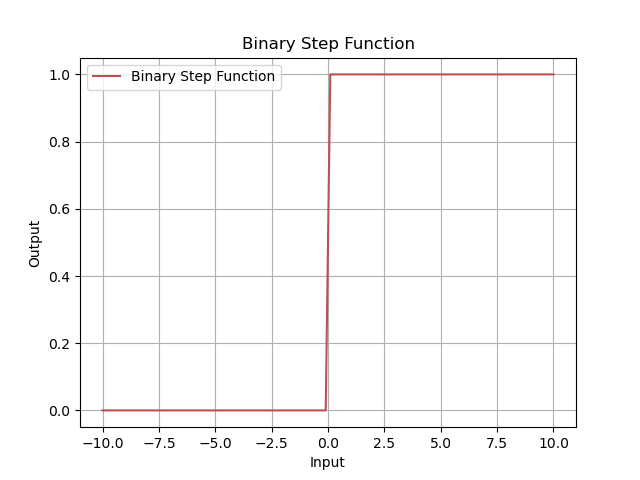
\includegraphics[width=\textwidth]{Figures/chapter_ne/ne_binary_step_plot.png} % Include the figure image
    \caption{Binary Step Activation Function Plot}
    \label{fig:ne_binary_step_plot} % Unique label used for referencing the figure in-text
\end{figure}

\parbreak\noindent \textbf{Linear Activation Function} (\textit{Linear Function Category}): This function represents a relationship that is directly proportional to the input. It is mathematically represented as shown in Equation \ref{alg:linear_function} and visually illustrated in Figure \ref{fig:ne_linear_plot} (\cite{sharma2017activation}). Linear activation functions are best suited for regression problems where linear relationships are the only concern (\cite{sharma2017activation}).
  
\begin{ceqn}
    \begin{equation}\label{alg:linear_function}
        f(x) = ax
    \end{equation}
\end{ceqn}

\parbreak
\begin{figure}[H] % Use [H] to suppress floating and place the figure/table exactly where it is specified in the text
    \centering % Horizontally center the figure on the page
     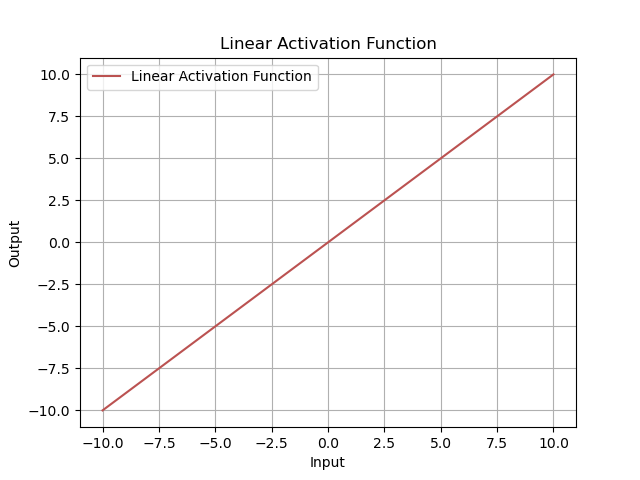
\includegraphics[width=\textwidth]{Figures/chapter_ne/ne_linear_plot.png} % Include the figure image
    \caption{Linear Activation Function Plot}
    \label{fig:ne_linear_plot} % Unique label used for referencing the figure in-text
\end{figure}

\parbreak\noindent \textbf{Sigmoid Activation Function} (\textit{Non-linear Function Category}): This function is the most widely used activation function due to its ability to be continuously differentiable and non-symmetric about zero meaning that the sign of all output values of neurons will be the same (\cite{sharma2017activation}). It is mathematically represented as shown in Equation \ref{alg:sigmoid_function} and visually illustrated in Figure \ref{fig:ne_sigmoid_plot} (\cite{sharma2017activation}). This activation function brings non-linearity into the neural network having applicability a wide range of tasks such as classification problems, function approximation, etc - essentially problems that involve complex relationships to be learned (\cite{sharma2017activation}).
    
\begin{ceqn}
    \begin{equation}\label{alg:sigmoid_function}
        f(x) = \frac{1}{e^{-x}}
    \end{equation}
\end{ceqn}

\parbreak
\begin{figure}[H] % Use [H] to suppress floating and place the figure/table exactly where it is specified in the text
    \centering % Horizontally center the figure on the page
    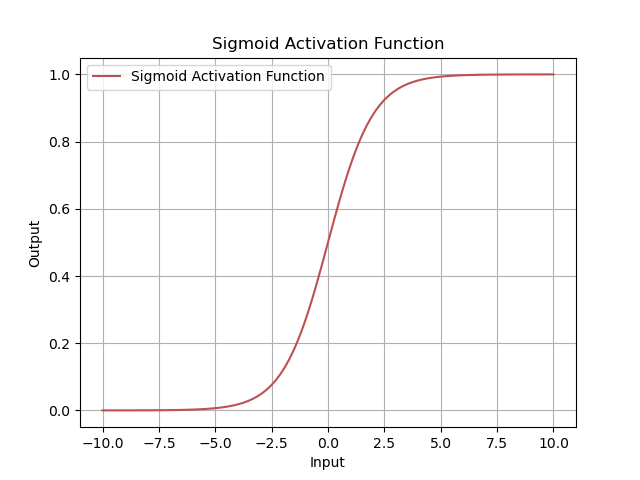
\includegraphics[width=\textwidth]{Figures/chapter_ne/ne_sigmoid_plot.png} % Include the figure image
    \caption{Sigmoid Activation Function Plot}
    \label{fig:ne_sigmoid_plot} % Unique label used for referencing the figure in-text
\end{figure}

\noindent There are many other popular activation functions that include \textit{ReLU}, \textit{LeakyReLU}, \textit{Hyperbolic Tangent}, and so on which each have their applicability in a particular task. Choosing the correct activation function has many considerations such as the number of hidden layers in the network, the training method used, hyperparameter tuning, etc. (\cite{sharma2017activation}).

\subsection{Backpropagation}
Backpropagation, short for backward propagation of errors, is a fundamental algorithm that is used to train neural networks. Traditionally in early years of artificial neural network research (1950s-1980s), the training of neural networks was not common and made the use of neural networks undesirable (\cite{aggarwal2018neural}). Since its introduction in the 1980s, backpropagation has become a cornerstone of modern deep learning (\cite{aggarwal2018neural}).

\parbreak\noindent Backpropagation's main concept is based on understand how changing the weights and biases in a network impacts the cost function (\cite{nielsen2015neural}). The cost function measures the network's overall performance across all training examples, serving as the optimisation target during learning. This differs from the loss function, which calculates the error for a single sample. The cost function aggregates these individual losses (typically through averaging) to guide weight adjustments across the entire dataset. The cost function is defined mathematically as (\cite{nielsen2015neural}):
\begin{ceqn}
    \begin{equation}\label{alg:cost_function}
        C = \frac{1}{2n}\sum_{x} ||y(x)-a^L(x)||^2
    \end{equation}
\end{ceqn}

\noindent where:
\begin{itemize}
    \item $n$ is the total number of training examples
    \item $x$ is the training individual example
    \item $y(x)$ is the desired output
    \item $a^L(x)$ is the vector of activation outputs when $x$ is the input
\end{itemize}

\parbreak\noindent There are four main equations that are needed for backpropagation to work (\cite{nielsen2015neural}):

\begin{enumerate}
    \item The first equation allows the computation of the error in output layer $L$:
    \begin{ceqn}
        \begin{equation}\label{alg:bp1}
            \delta^L = \nabla_aC\odot\sigma'(z^L)
        \end{equation}
    \end{ceqn}
    \noindent where:
    \begin{itemize}
         \item $\delta^L$ is the error in output layer $L$
        \item $\nabla_aC$ is a vector whose components are the partial derivatives $\frac{\partial C}{\partial a_j^L}$ - in other words, the rate of change of C with   respect to the output activation
        \item $\odot$ is the elementwise multiplication operator
        \item $\sigma'(z_J^L)$ measures how fast the activation function $\sigma$ changes at $z_j^L$
        \item $z_j^l$ is the weighted input of neuron $j$ at layer $l$
    \end{itemize}

    \item The second equation allows the computation of the error $\delta^l$ in terms of the error in the following layer:
    \begin{ceqn}
        \begin{equation}\label{alg:bp2}
            \delta^l = ((w^{l+1})^T\delta^{l+1})\odot\sigma'(z^l)
        \end{equation}
    \end{ceqn}
    \noindent where:
    \begin{itemize}
        \item $\delta^l$ is the error in the next layer
        \item $(w^{l+1})^T$ is the transpose of the weight matric $w^{l+1}$ for the $(1+l)$-th layer
    \end{itemize}

    \item Equation \ref{alg:bp1} and \ref{alg:bp2} can be combined to provide the third main equation of backpropagation which allows the computation of the error $\delta^l$ for any layer in the network:
    \begin{ceqn}
        \begin{equation}\label{alg:bp3}
            \frac{\partial C}{\partial b_j^l} = \delta_j^l
        \end{equation}
    \end{ceqn}

    \item The fourth and final equation allows the computation of partial derivatives $\frac{\partial C}{\partial w_{jk}^l}$ in terms of $\delta^l$ and $a^{l-1}$:
    \begin{ceqn}
        \begin{equation}\label{alg:bp4}
            \frac{\partial C}{\partial w_{jk}^l} = a_k^{l-1}\delta_j^l
        \end{equation}
    \end{ceqn}
\end{enumerate}

\parbreak\noindent With the above four main equations in mind, the backpropagation algorithm works as follows:

\begin{algorithm}[H]
	\caption{Basic Backpropagation Algorithm (\cite{nielsen2015neural})}\label{alg:backpropogation_algorithm}
	\begin{algorithmic}[1]
    \item \textbf{Input} value x: Set the corresponding activation $a^1$ for the input layer
    \item \textbf{Feedforward}: For each layer, $l=1,2,3,...,L$, compute the weighted sum $z^l=w^la^{l-1}+b^l$ and the activation value $a^l=\sigma(z_l)$
	\item \textbf{Output error} $\delta^L$: Compute the error of the output layer using $\delta^L=\nabla_aC\odot\sigma'(z^L)$ (Equation \ref{alg:bp1})
	\item \textbf{Backpropagate the error}: For each layer, $l=L-1, L-2,...,2$, computer the error for that layer using $\delta^l=((w^{l+1})^T\delta^{l+1}) \odot\sigma'(z^l)$ (Equation \ref{alg:bp2})
	\item \textbf{Output}: The gradient of the cost function is given by $\frac{\partial C}{\partial b_j^l} = \delta_j^l$ and $\frac{\partial C}{\partial w_{jk}^l} = a_k^{l-1}\delta_j^l$ (Equation \ref{alg:bp3} and \ref{alg:bp4} respectively)
\end{algorithmic}
\end{algorithm}

\parbreak\noindent In essence, the backpropogation algorithm computes the gradient of the loss function with respect to each weight in the network for a single training example, however, calculating these gradients alone does not update the network. To actually train the model, backpropagation is typically combined with an optimisation algorithm such as stochastic gradient descent (SGD). Gradient descent uses the computed gradients to iteratively adjusts the weights in a direction that minimises the overall cost function. In the case of SGD, this process is performed using small batches or individual training examples, which allows for faster and more scalable learning. This combination of backpropagation and gradient descent forms the foundation of most conventional neural network training mechanisms (\cite{nielsen2015neural}).

\section{Neural Architecture Search}\label{sec:ne_nas}
Neural Architecture Search (NAS) is a technique in artificial intelligence aimed at automating the design of neural network architectures as opposed to the traditional method of crafting these neural networks by hand and through trial-and-error, both of which are time-consuming and prone to suboptimal outcomes (\cite{ren2021comprehensive}). NAS addresses these challenges by employing algorithms to discover optimal or near-optimal architectures tailored for a specific task. NAS represents a significant shift towards making machine learning more scalable and accessible, bridging the gap between model development and deployment (\cite{elsken2019neural}).

\parbreak\noindent NAS is based on three core components and are combined to form the NAS methods illustrated in Figure \ref{fig:ne_nas}. (\cite{elsken2019neural}):

\begin{itemize}
    \item \textbf{Search Space}: This component defines the set of possible neural network architectures that NAS can explore and includes various design elements such as layer types, number of layers, connectivity patterns, and the neural networks hyperparameters. A well-structured search space is extremely important as it balances between being expressive enough to capture high-performing architectures while still being constrained enough to allow efficient exploration (\cite{elsken2019neural}).
    \item \textbf{Search strategy}: This component dictates how the NAS algorithm navigates the search space to identify optimal architectures. Common search strategies include reinforcement learning, evolutionary algorithms, and gradient-descent methods (\cite{liu2021survey}). Reinforcement learning makes use of a controller model to generate architectural decisions, while evolutionary algorithms mimic natural selection by evolving a population of candidate architecture solutions over successive generations. Gradient-based approaches, such as Differentiable Architecture Search (DARTS), enable more efficient exploration by allowing continuous relaxation of the search space (\cite{liu2021survey}).
    \item \textbf{Performance Estimation Strategy}: This component assesses how promising a candidate architecture is without fully training it, which is essential due to the high computation cost involved in evaluating each neural network design (\cite{elsken2019neural}). Techniques like early stopping, weight sharing, and surrogate models are used to estimate performance more efficiently (\cite{elsken2019neural}).
\end{itemize}

\parbreak
\begin{figure}[H] % Use [H] to suppress floating and place the figure/table exactly where it is specified in the text
	\centering % Horizontally center the figure on the page
	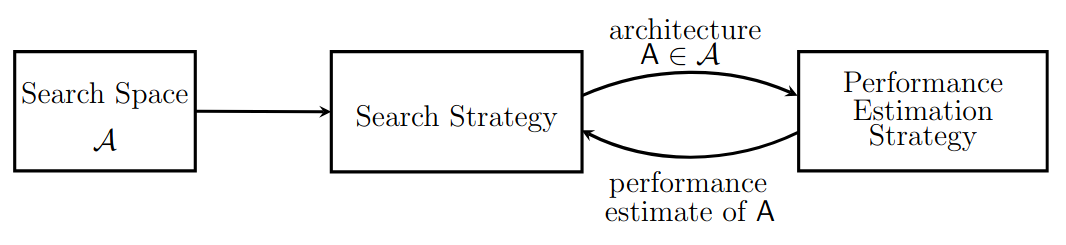
\includegraphics[width=\textwidth]{Figures/chapter_ne/ne_nas.png} % Include the figure image
	\caption{Neural Architecture Search methods framework (\cite{elsken2019neural})}
	\label{fig:ne_nas} % Unique label used for referencing the figure in-text
\end{figure}

\parbreak\noindent NAS has evolved through the development of many methods, each offering distinct approaches in navigating the search space. One prominent approach is \textbf{reinforcement learning-based} learning, where the generation of a neural network architecture is considered an agent's action and the agent's reward correlated to the performance of a trained architecture on unseen data (\cite{elsken2019neural}). The most influential method is \textbf{evolutionary algorithms} (mentioned in Chapter \ref{chapter_ea}) which mimics biological evolution by iteratively apply genetic operators and selecting high-performing architectures. This approach is highly adaptive however can also become computationally intensive fast. More recently, \textbf{gradient-based} NAS methods as mentioned previously have gained popularity for their efficiency. DARTS for example, relaxes the discrete search space into a continuous one enabling gradient descent optimization to find optimal architectures far quicker and with reduced computational demands (\cite{liu2021survey}). These methods differ in scalability, model performance, and efficiently. Reinforcement learning and evolutionary algorithms excel in finding innovative architectures but are computationally expensive while gradient-based approaches offer faster and more resource-efficient search offering more practical application, however, do not innovate as well (\cite{elsken2019neural}).

\parbreak\noindent Despite the promising potential that NAS provides, it still faces several significant challenges. The most pressing issue is its high computational cost (\cite{liu2021survey}). Traditional NAS methods, especially those making use of reinforcement learning and evolutionary algorithms require the training of thousands of candidate models, consuming computational resources and time exponentially, making NAS undesirable to researchers and organizations with limited infrastructure (\cite{elsken2019neural}). Another issue lies in the design of the search space. Creating a search space that is both expressive and efficient becomes a complex task. A poorly designed search space can either be to restrictive hindering exploration, or too expensive leading to inefficient searches and suboptimal models (\cite{liu2021survey}).

\parbreak\noindent Recent advancements in NAS have focused on mitigating the challenge of computational demands and improving generalization. One notable development is the use of weight sharing whereby multiple candidate solution architectures share parameters during training. This technique significantly reduces the time needed to train each model therapy cutting computational demands (\cite{pham2018efficient}). Another advancement in the field of NAS is the aforementioned DARTS technique which transforms the discrete search space in a continuous one, allowing for architecture parameters to be optimized efficiently using gradient descent based methods and thereby enhancing the search speed and reducing resource consumption (\cite{liu2021survey}). Additionally, strategies like proxy models and early stopping have been employed to estimate model performance without fully training each candidate solution architecture, helping mitigate excessive computation while still allowing for the consideration of innovative architectures (\cite{liu2021survey}). NAS has also extended into real-world application such as computer vision whereby NAS-designed models have achieved state-of-the-art results in image classification and object detection. In natural language processing, NAS has contributed to more efficient transformer architectures, optimizing performance for tasks such as text generation and machine translation (\cite{elsken2019neural}).


\section{Neuroevolution of Augmenting Topologies}\label{sec:ne_neat}
\subsection{Introduction to NEAT}
The Neuroevolution of Augmenting Topologies (NEAT) algorithm is a pioneering method in neuroevolution, known for its powerful ability evolve both the structure and weights of a neural network (\cite{stanley2019designing}). NEAT begins with simple networks and gradually increases its complexity through evolutionary principles. It is based on three core principles in an attempt to solve the challenges that topology and weight evolving artificial neural networks (TWEANNs) face, namely, (1) its unique genetic encoding scheme, (2) mechanism of speciation, and (3) minimization of dimensionality through incremental growth from minimal structures (\cite{stanley2002evolving}).

\parbreak
\begin{figure}[H] % Use [H] to suppress floating and place the figure/table exactly where it is specified in the text
	\centering % Horizontally center the figure on the page
	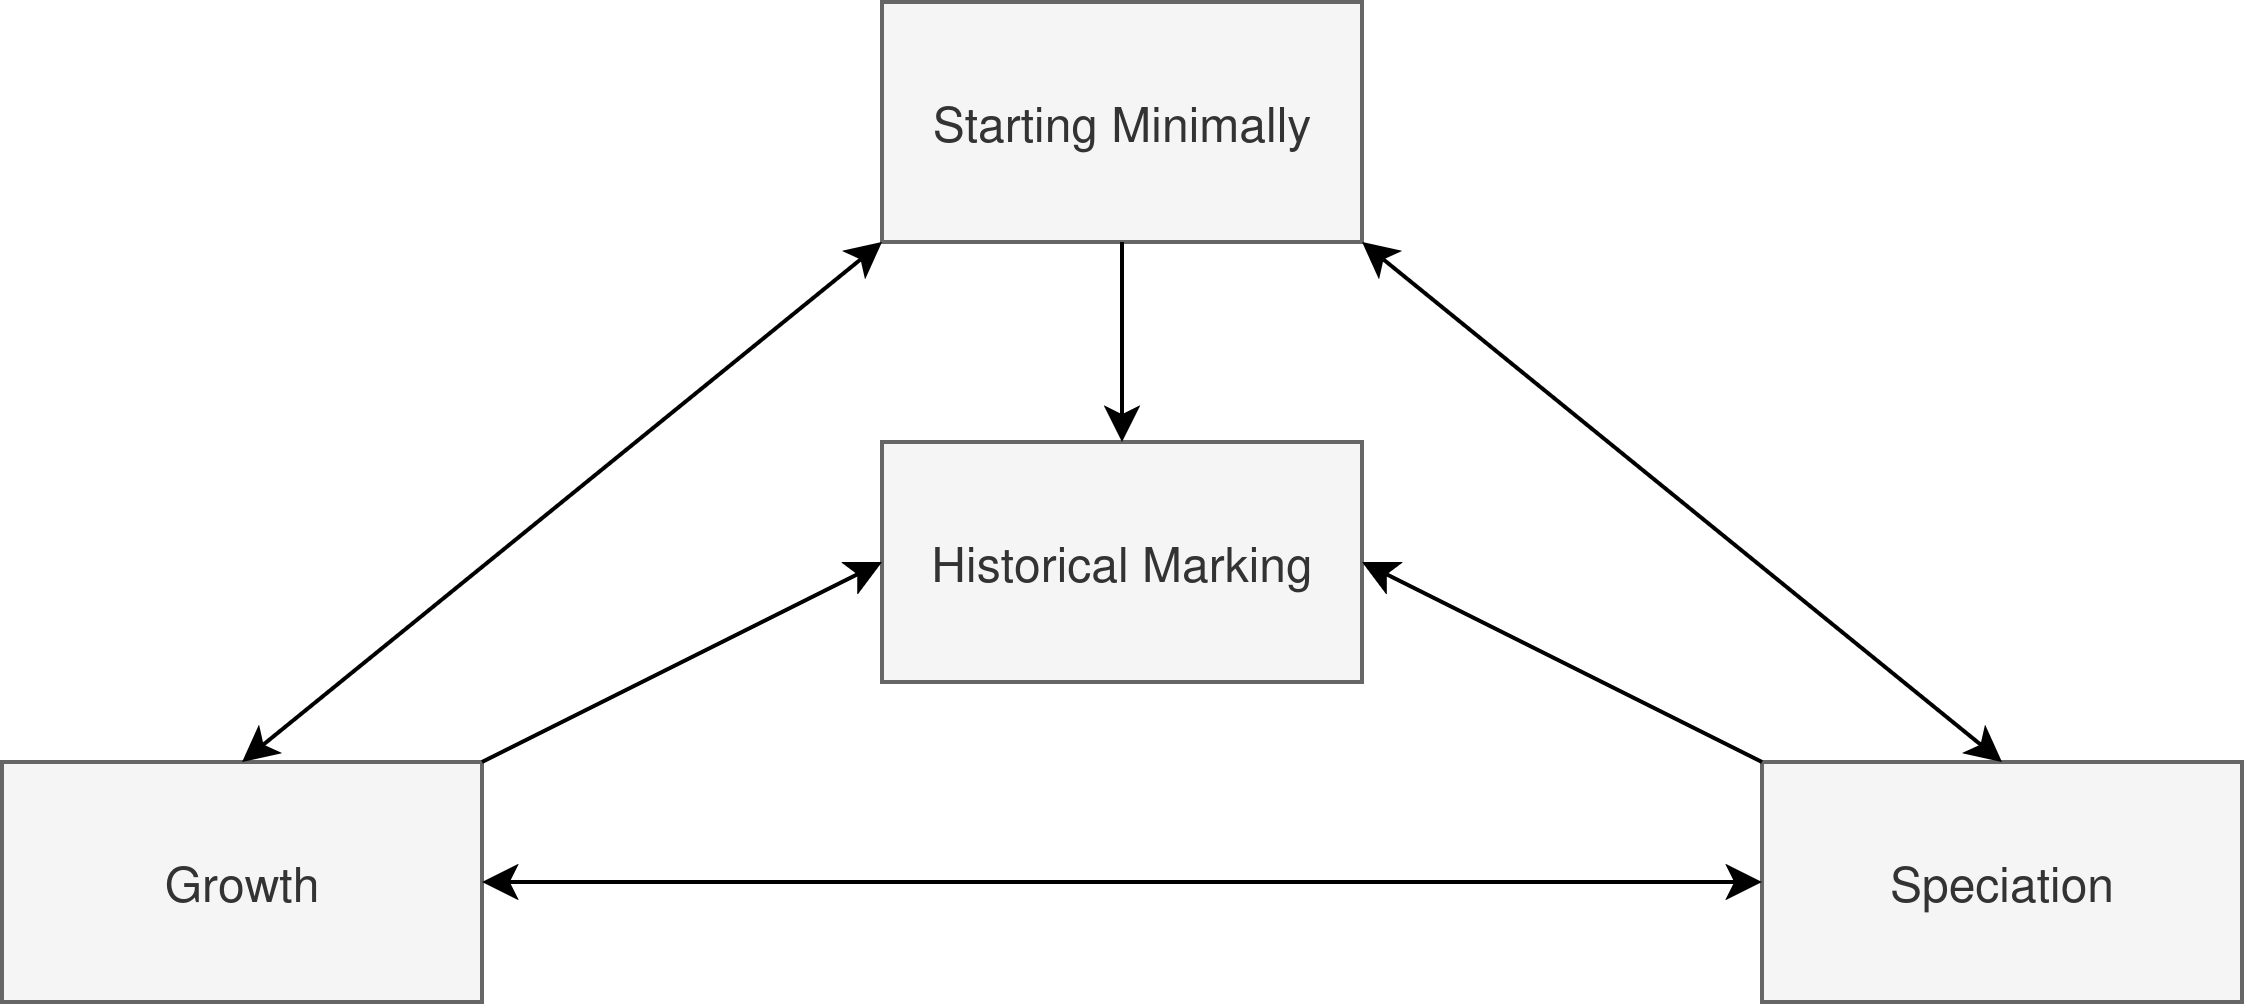
\includegraphics[width=\textwidth]{Figures/chapter_ne/ne_neat_components.png} % Include the figure image
	\caption{NEAT Component Dependencies (adapted from \cite{stanley2002evolving})}
	\label{fig:neat_depedencies} % Unique label used for referencing the figure in-text
\end{figure}

\parbreak\noindent Genetic encoding allows the transformation between phenotype, being the actual neural network representation, to genotype, being a linear string subject to genetic operators. Mutations to these genotypes introduce changes such as the addition of new nodes, altered weights, or additional connections, while crossover operations combine features from parent neural networks. These genetic operations are tailored in such away that functional integrity is maintained, ensuring that the offspring networks inherit the best traits. Importantly, NEAT aims to solve the issue of competing conventions whereby candidate solutions can possibly represent the same outcome even though they have different gene configurations. With reference to Figure \ref{fig:competing_convension}, the crossover between two neural networks that are identical representations but are just different structure configurations can lead to a loss in information (\cite{stanley2002evolving}). This challenge stems from the isomorphism problem, where functionally equivalent networks may have different node and connection patterns, making meaningful genetic recombination difficult.

\parbreak
\begin{figure}[H] % Use [H] to suppress floating and place the figure/table exactly where it is specified in the text
	\centering % Horizontally center the figure on the page
	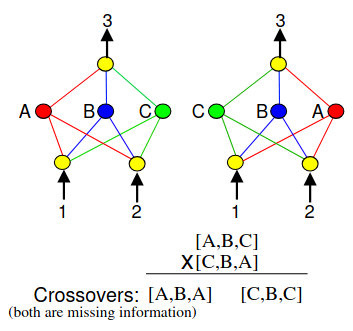
\includegraphics[width=\textwidth]{Figures/chapter_ne/ne_competing_convention.png} % Include the figure image
	\caption{Competing Convention between Neural Network Solutions (adapted from \cite{stanley2002evolving})}
	\label{fig:competing_convension} % Unique label used for referencing the figure in-text
\end{figure}

\parbreak\noindent Speciation preserves unique structures by grouping similar networks into species, protecting novel characteristics from premature elimination. This mechanism prevents innovative offspring from being directly compared with established and well performing networks, which might otherwise out compete them prematurely. By fostering innovation within smaller networks, speciation allows NEAT to better exploit the search space and void stagnation (\cite{stanley2002evolving}). While speciation mechanisms exist across evolutionary algorithms (as mentioned in Chapter \ref{chapter_ea}), NEAT implements this through its distinctive approach of historical markings and compatibility distance, which constitutes its key innovation.

\parbreak\noindent Incremental growth refers to the gradual introduction of nodes and connections through subsequent generations, enabling networks to evolve complexity only when advantageous. This approach avoids computational overhead when dealing with unnecessarily complex networks in early stages and ensures that the algorithm uses these networks as core building blocks in creating innovative candidate solutions (\cite{stanley2002evolving}).

\subsection{Mechanics of NEAT}
\subsubsection{Initialisation of Population}
The mechanics of NEAT rely on sophisticated yet efficient process that balance exploration and exploitation in evolving neural networks. The algorithm begins with a population of minimal neural networks, typically consisting of input and output nodes without hidden layers. This simplicity is intentional, as NEAT focuses on incremental growth by introducing new nodes and connection only when they enhance the networks performance. The reason being is that networks that are randomly generated and complex tend to go through the effort of removing connections and nodes that are not needed in the first place (\cite{stanley2002evolving}). NEAT's initialisation scheme prevents modifications where fitness functions track network size, as this would unnecessarily complicate fitness evaluation. Starting out minimally ensures that candidate solutions explore the search space in the lowest dimensional weight space first, resulting in dramatic performance gains early on. Another added advantage of starting out simply is the manifestation of speciation. Starting out simply and complexifying over subsequent generations aligns with Darwinian principles (\cite{stanley2002evolving}).

\subsubsection{Phenotype-Genotype Mapping}
NEAT's genetic encoding scheme is designed in such away that allows genetic operations to be performed without leading to non-functional neural networks, a problem that traditional TWEANNs face. The neural network (phenotype) is encoded in a linear representation as shown in Figure \ref{fig:genotype_phenotype_neat_mapping}.

\parbreak
\begin{figure}[H] % Use [H] to suppress floating and place the figure/table exactly where it is specified in the text
	\centering % Horizontally center the figure on the page
	\includesvg[width=\textwidth]{Figures/chapter_ne/ne_genotype_mapping.svg} % Include the figure image
	\caption{NEAT's Genotype-Phenotype Mapping (adapted from \cite{stanley2002evolving})}
	\label{fig:genotype_phenotype_neat_mapping} % Unique label used for referencing the figure in-text
\end{figure}

\parbreak\noindent The mapping works by assigning each node in the neural network representation with an index. The genome of the genotype representation is made up of \textit{node genes} and \textit{connection genes}. Node genes represents input, hidden, and output nodes that make up the network whereas connection genes specify the following information:

\begin{itemize}
    \item \textbf{In}: The outgoing connection of the node.
    \item \textbf{Out}: The incoming connection of the node.
    \item \textbf{Weight}: The weight of the connection.
    \item \textbf{Enabled}: Dictates whether the connection is active or not.
    \item \textbf{Innov}: Serves as a historical marker in tracking corresponding genes.
\end{itemize}

\subsubsection{Genetic Operators}
\noindent NEAT makes use of both mutation and crossover to produce viable offspring. Mutation has the ability to change both the connection weights and network structures. Weight mutation works as normal in any evolutionary algorithm whereby the mutation value is chosen and changed according to some function as explained in Section \ref{label:ea_genetic_operators}. Structural mutations can occur in two ways, each of which expands the size of the genome (\cite{stanley2002evolving}):
\begin{itemize}
    \item \textbf{Add connection} mutation: This mutation adds a single new connection between two previously unconnected nodes. Figure \ref{fig:neat_add_connection} illustrates this by mutating the genome such that a connection is formed between node 1 and 4.
    \item \textbf{Add node} mutation: This mutation splits an existing connection and places a new node where this existing connection use to be. This involves the old connection being disabled. The new connection leading from the old node into the new node receives a weight of 1 while the new connection leading from the new into the other old node receives the same weight as the old connection. Figure \ref{fig:neat_add_node} illustrates this by mutating the genome such that node 6 is added, with two new connections forming between node 1 and 6, and node 6 and 5.
\end{itemize}

\parbreak\noindent This mutation mechanism allows the initial effect of mutation to be minimised. In traditional mutations as those seen in genetic programming which allows extraneous structures to be added, NEAT essentially forces the structures to be evolved in complex ways later on allowing the network to exploit simple structures first (\cite{stanley2002evolving}). The crossover genetic operator is applicable in NEAT as well, however, enabled through a mechanism known as gene tracking through historical markings.

\parbreak
\begin{figure}[H] % Use [H] to suppress floating and place the figure/table exactly where it is specified in the text
	\centering % Horizontally center the figure on the page
	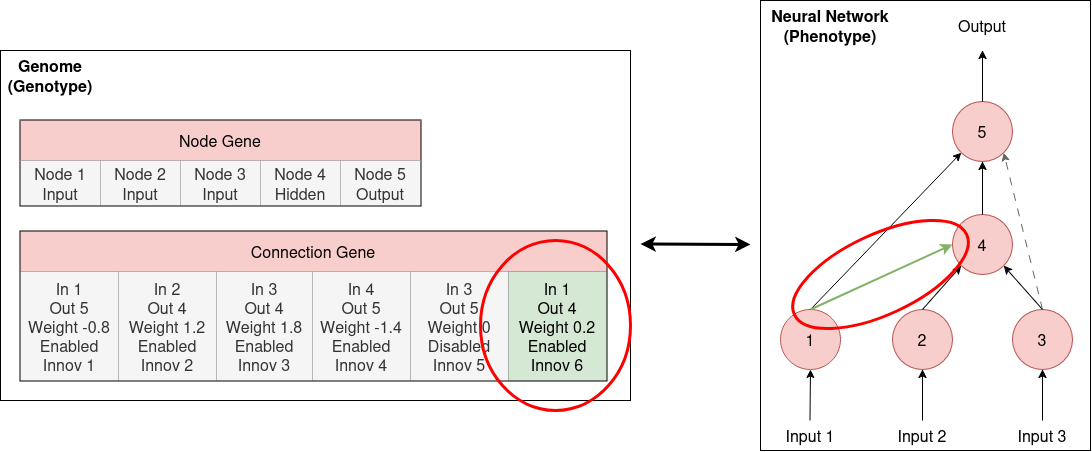
\includegraphics[width=\textwidth]{Figures/chapter_ne/ne_add_connection.png} % Include the figure image
	\caption{NEAT's Add Connection Mutation Mechanism (adapted from \cite{stanley2002evolving})}
	\label{fig:neat_add_connection} % Unique label used for referencing the figure in-text
\end{figure}

\parbreak
\begin{figure}[H] % Use [H] to suppress floating and place the figure/table exactly where it is specified in the text
	\centering % Horizontally center the figure on the page
	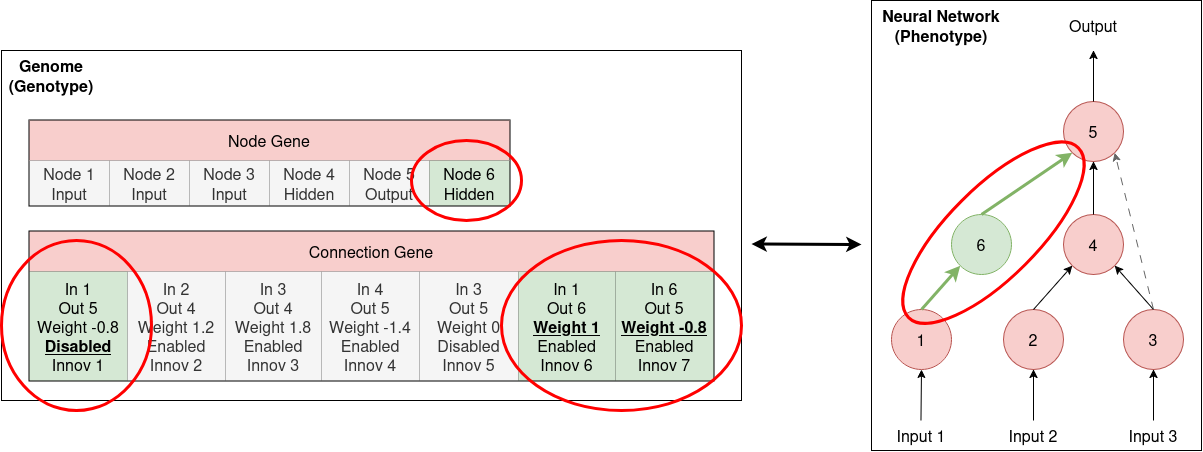
\includegraphics[width=\textwidth]{Figures/chapter_ne/ne_add_node.png} % Include the figure image
	\caption{NEAT's Add Node Mutation Mechanism (adapted from \cite{stanley2002evolving})}
	\label{fig:neat_add_node} % Unique label used for referencing the figure in-text
\end{figure}

\subsubsection{Historical Markings}
Historical markings is a powerful capability of NEAT that solves the problem of competing conventions. Innovation numbers that are seen in Figure \ref{fig:genotype_phenotype_neat_mapping} enables this capability and represents a chronology of the appearance of every gene. When the initial population is generated, a unique innovation number is assigned to every unique connection. When a new gene appears, a \textit{global innovation number} is incremented and assigned to that gene. 

\parbreak
\begin{figure}[H] % Use [H] to suppress floating and place the figure/table exactly where it is specified in the text
	\centering % Horizontally center the figure on the page
	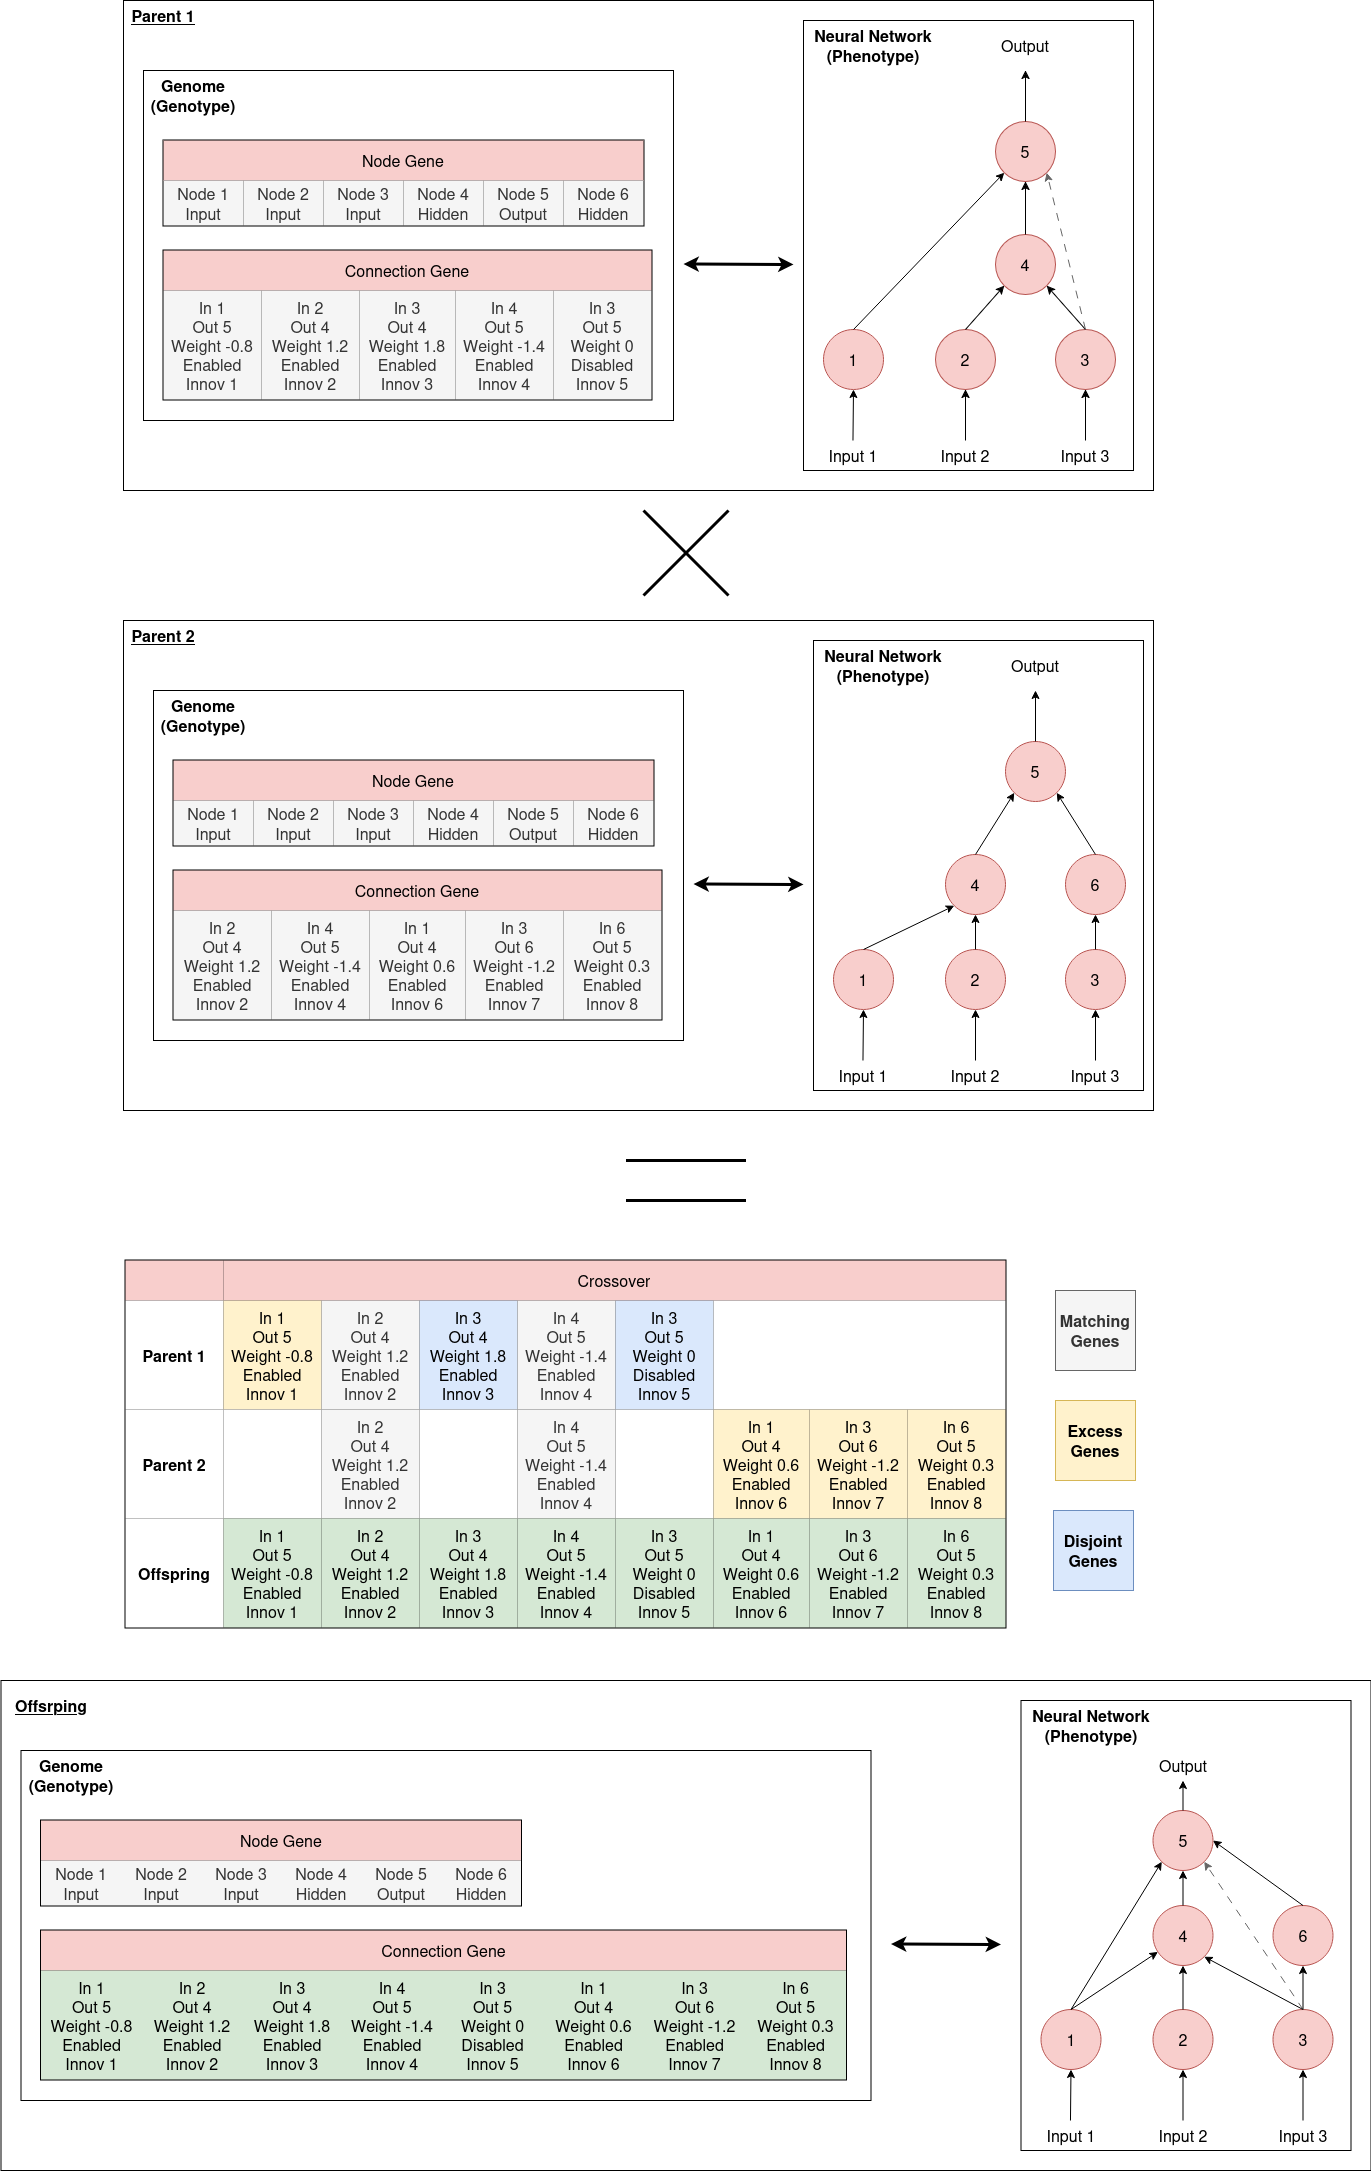
\includegraphics[width=\textwidth]{Figures/chapter_ne/ne_neat_crossover.png} % Include the figure image
	\caption{NEAT's Crossover Mechanism (adapted from \cite{stanley2002evolving})}
	\label{fig:neat_crossover} % Unique label used for referencing the figure in-text
\end{figure}

\parbreak\noindent There might be a chance mutations may result in the same structural innovation amongst multiple candidate solutions within a generation - to avoid assigning different innovation numbers in this scenario, a list of gene innovations are kept for that generation meaning that if mutations result in the same structural innovation amongst multiple genes, they receive the same innovation number.

\parbreak\noindent Importantly, tracking the historical markings of genes provides a way to exactly know which genes match up when performing crossover. Genes that line up according to their \textit{innovation number} are called \textit{matching} genes. Genes that do not split are categorized as either \textit{disjoint} or \textit{excess} depending what their positions are with regard to the other parent. For example, in Figure \ref{fig:neat_crossover}, gene 4 to 6 of parent 1, and gene 1 to 4 of parent 2 form disjoint genes while gene 7 to 8 of parent 2 form genes that are in excess. Matching genes up in this fashion using innovation allows crossover to happen naturally.

\subsubsection{Speciation}
Speciation was introduces in NEAT to allow candidate solutions to compete primarily within their own niches as opposed to the entire population. Doing this means that new topological innovations are protected in a new niche allowing them to optimize through competition within the niche. The idea behind this is to prevent premature convergence and stagnation allowing candidate solutions to exploit the search space thoroughly. Speciating is efficiently enabled through innovation numbers by comparing how many disjoint genes there are between candidate solutions. Essentially, the more disjoint two genomes are, the less historical markers they share and by that extent are less compatible (\cite{stanley2002evolving}). This compatibility can be calculated through the following mathematical equation (\cite{stanley2002evolving}):
\begin{ceqn}
    \begin{equation}\label{alg:speciation}
        \delta = \frac{c_1E}{N} + \frac{c_2D}{N} + c_3\cdot{\overline{W}}
    \end{equation}
\end{ceqn}

\noindent where:
\begin{itemize}
    \item $\delta$ is the compatibility distance between a pair of genomes
    \item $E$ is the number of excess genes
    \item $D$ is the number of disjoint genes
    \item $\overline{W}$ is the average weight difference of matching genes
    \item $N$ is the number of genes in the larger genome (serving as a normalization)
    \item $c_1$, $c_2$, and $c_3$ serve as adjustments in the importance of the three factors
\end{itemize}

\parbreak\noindent The compatibility distance, $\delta$, allows speciation using a threshold $\delta_t$. During the evolution process, a list of species is maintained, and candidate solutions are speciated in each generation. A species is represented by a random genome inside that species known as the \textit{species representative}. Given a genome $g$ in a generation, it is placed in the first species that it is found to be compatible within the species representative of that species - if no species is found, it forms part of a new species (\cite{stanley2002evolving}).

\parbreak\noindent Species have the benefit of having access to all candidate solution's fitness function values within that species during reproduction which is a mechanism known as \textit{explicit fitness sharing}. This means that a single candidate solution is unlikely to dominate the species. Speciation involves an adjusted fitness functions as follows (\cite{stanley2002evolving}):
\begin{ceqn}
    \begin{equation}\label{alg:speciation}
        f'_i = \frac{f_i}{\sum_{j=1}^{n}sh(\sigma(i,j))}
    \end{equation}
\end{ceqn}

\noindent where:
\begin{itemize}
    \item $f'_i$ is the fitness of candidate solution $i$
    \item $f_i$ is the chosen fitness function for the neural network
    \item $\sigma(i,j)$ is the compatibility distance seen in Equation \ref{alg:speciation} between organism $i$ and $j$
    \item $sh$ is the sharing function that operates as follows:
    \begin{ceqn}
        \begin{equation}\label{alg:sharing_function}
            sh(\sigma(i,j)) = 
            \begin{cases} 
                1 \:\: if \:\: \delta(i,j) > \delta_t \\
                0 \:\: otherwise
            \end{cases}
        \end{equation}
    \end{ceqn}

    \item $\sum_{j=1}^{n}sh(\sigma(i,j))$ reduces to the number of candidate solutions in the same species as candidate solution $i$
\end{itemize}

\parbreak\noindent Making use of this adjusted fitness function means that species reproduce by first eliminating the weakest links. Speciating the population in this regard ensures that the topological innovation is protected.

\subsubsection{Minimizing Dimensionality}
The last core concept in NEAT is its minimization in dimensionality through incremental growth from minimal structures. When initializing the population at the start of the algorithm, NEAT biases its search around minimal dimensional spaces by initializing candidate solutions with zero hidden nodes. As subsequent generations occur, new structures are introduced incrementally by means of mutation and crossover. This means that the topology innovations that occur are justified. Due to starting out minimally, NEAT outperforms other TWEANN based search algorithms requiring fewer dimension to find optimal solutions (\cite{stanley2002evolving}).

\subsection{Strengths and Challenges of NEAT}
The NEAT algorithm has several strengths that have contributed to its widespread use in artificial intelligence research. One of its primary advantages is its efficiency in evolving neural network with minimal complexity. When applied to the double pole balancing problem, NEAT was able to find an optimal solution in as little as 24 generations made up of 150 nodes, a network far more minimal than other traditional TWEANNs (\cite{stanley2002evolving}). By starting out with simple networks and adding complexity gradually, NEAT avoids the inefficiencies associated with random initialisation of large, complex networks. This makes NEAT particularly suitable for tasks where the optimal topology is unknown.

\parbreak\noindent Another strength of NEAT is its ability to preserve diversity within the population by means of its speciation algorithm which ensures that innovative solutions are no prematurely discarded, allowing the algorithm to explore a wide range of architectures. In the original paper of NEAT, to understand the importance of speciation, a graph was produced to illustrate how speciation impacts innovation which is shown in Figure \ref{fig:neat_speciate_vis}. As subsequent generations occur, species guide their search collectively towards an optimal solution showcasing its thorough search capability. Fitness sharing within species also prevents over-optimization of a single solution thereby fostering more robust search process. These features make NEAT well-suited for solving complex and high-dimensional problems (\cite{stanley2002evolving}). 

\parbreak
\begin{figure}[H] % Use [H] to suppress floating and place the figure/table exactly where it is specified in the text
	\centering % Horizontally center the figure on the page
	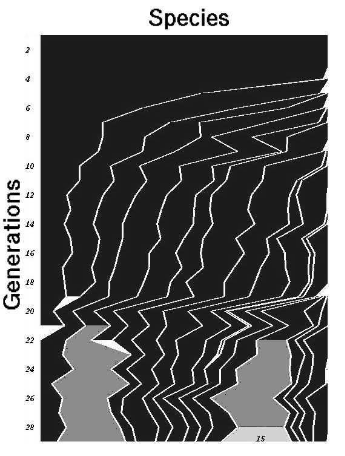
\includegraphics[width=0.50\textwidth]{Figures/chapter_ne/ne_neat_speciate_vis.png} % Include the figure image
	\caption{Visualizing NEAT's Speciation Mechanism while Solving the Double Pole Balancing Problem (\cite{stanley2002evolving})}
	\label{fig:neat_speciate_vis} % Unique label used for referencing the figure in-text
\end{figure}

\parbreak\noindent Additionally, NEAT offers significant advantage over traditional gradient-based methods, that is, it does not require the objective function or for the resulting neural network to be differentiable. While conventional training relies on backpropagation and gradient descent, NEAT evaluates candidate networks based soley on their performance. This makes it applicable to a wider range of problems, including those with discrete, noisy, or non-differentiable environments (\cite{stanley2002evolving}). As a result, NEAT provides greater flexibility in domains where gradient information is unreliable or simply unavailable.

\parbreak\noindent Despite its strengths, NEAT faces several challenges. One of the most significant is its computational costs. The simultaneous evolution of topology and weights requires high computation feature extraction (\cite{peng2018neat}). Additionally, because NEAT evolves arbitrary network topologies rather than layered architectures, it cannot leverage efficient matrix operations for forward propagation. Instead, each neuron must be activated individually following a topological sort, resulting in slower network evaluation. Another challenge is the sensitivity in fine-tuning the hyperparameters such as the mutation rates, speciation thresholds, and population size. Improper tuning can lead to issues such as stagnation, overfitting, or excessive computational overhead (\cite{stanley2002evolving}).

\parbreak\noindent Overall, NEAT's strengths far outweigh its limitations, particular in optimization problems requiring innovative architectures or dynamic adaptability. As computational resources improve, many of NEAT's challenges may become less significant, further establishing its role as a powerful tool in neuroevolution.

\subsection{HyperNEAT, a NEAT extension}
Hypercube-based Neuroevolution of Augmenting Topologies (HyperNEAT), an extension of NEAT was developed to address the challenges in problems with inherent geometric or spacial structures. While NEAT excels at evolving neural networks by optimizing both topology and weights, it does not necessarily exploit the spatial relationships present in real-world tasks such as image recognition (\cite{stanley2009hypercube}). HyperNEAT extends NEAT by introducing an indirect encoding mechanisms using Compositional Pattern Producing Networks (CPNNs), which represent neural network connectivity patterns as mathematical functions.

\parbreak\noindent CPPNs allow HyperNEAT to encode complex patterns of connectivity in a compact fashion. Instead of explicitly defining each connection, CPPNs describe how connections between neurons should be formed based on their geometric position. This approach is particularly advantageous for large-scale networks, where explicitly encoding all connection would be computationally prohibitive. HyperNEAT generates neural networks that are not only scalable but also better suited to exploit the inherent spatial structure of the task (\cite{stanley2009hypercube}).

\parbreak\noindent CPPNs can be thought of as a phenotype that is a pattern in space. Each coordinate in that space represents some level of expression as an output of a function that encodes the phenotype. The CPPN is a neural network that takes in coordinates and outputs a weight value which maps to a plane as shown in Figure \ref{fig:ne_hyperneat_cppn}. HyperNEAT revolves around three main steps, namely, substrate creation, CPPN evolution, and phenotype generation. The HyperNEAT algorithm is shown in Algorithm \ref{alg:hyperneat_algorithm}.

\parbreak\noindent \paragraph{Substrate Creation} involves the creation of a substrate which is a geometric representation of the neural network, where are nodes are arranged in such a way that reflects the spatial relationship inherent in the task (\cite{stanley2009hypercube}). For example, in robotic control tasks, the substrate might reflect the physical layout of sensors and actuators while in image recognition tasks the substrate might be a grid corresponding to pixel locations.

\parbreak\noindent \paragraph{CPPN Evolution} involve evolving CPPN networks using the NEAT algorithm. As mentioned, unlike a direct encoding where each connection is explicitly represented, the CPPN operates as a compact function that spits out weight values based on the relationship of underlying nodes in question. The CPPN's evolution is guided by a fitness function that evaluates the performance of the networks generated by the pattern encoded as a result from the CPPN (\cite{stanley2009hypercube}).

\parbreak\noindent \paragraph{Phenotype Generation} is the creation of the phenotype (the actual neural network) by querying the evolved CPPN for each pair of nodes in the substrate. For every set of nodes, the CPPN takes their spatial coordinates as inputs and returns a weight  representing the connections characteristics such as the weight values, whether they exist or not, etc. CPPN is essentially the blueprint that maps out the phenotype (\cite{stanley2009hypercube}). The resulting networks inherit the regularities encoded by the CPPN which allows them to better integrate unseen data based on their spatial relationship.

\parbreak
\begin{figure}[H] % Use [H] to suppress floating and place the figure/table exactly where it is specified in the text
	\centering % Horizontally center the figure on the page
	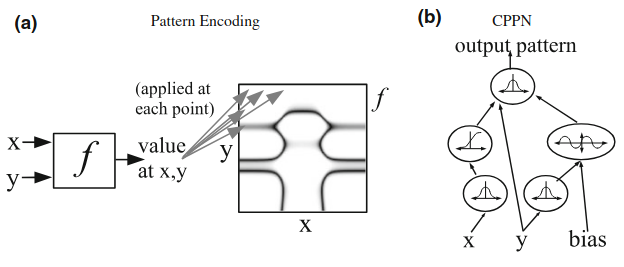
\includegraphics[width=\textwidth]{Figures/chapter_ne/ne_hyperneat_cppn.png} % Include the figure image
	\caption{CPPN encoding where \textbf{a} represents the pattern encoding as a result from output of the CPPN in \text{b} (\cite{d2014hyperneat})}
	\label{fig:ne_hyperneat_cppn} % Unique label used for referencing the figure in-text
\end{figure}

\begin{algorithm}[H]
	\caption{HyperNEAT algorithm (\cite{stanley2009hypercube})}\label{alg:hyperneat_algorithm}
	\begin{algorithmic}[1]
        \item Choose substrate configuration (i.e, node layout and input-output assignments)
        \item Initialize the poopulation of minimal CPPNs with random weights
        \item Repeat until a solution is found:
        \item \:\: For each member of the population
        \item \:\:\:\: Query its CPPN for the weight of each other connection in the substrate. If the absolute value of the output exceeds a threshold magnitude, create the connection with a weight scaled proportionally to the output value
        \item \:\:\:\: Run the substrate as an ANN in the task domain to ascertain fitness
        \item \:\: Reproduce the CPPNs according to the NEAT method to produce the next generation population
    \end{algorithmic}
\end{algorithm}

\parbreak\noindent One of HyperNEAT's notable strength resides in its ability to produce networks with inherent symmetries and patterns that mirror the problem domain (which is shown in Figure \ref{fig:ne_hyperneat_cppn}). This ability to capture and leverage geometric regularities makes HyperNEAT desirable in domains where spatial relationships are crucial. Although powerful, HyperNEAT can suffer from computational overhead, especially during the querying process of the CPPN to produce neural network solutions of a large scale (\cite{stanley2009hypercube}). Applications where HyperNEAT has been used include training agents to play games, learning autonomous agent controllers, robocup simulations, etc (\cite{kowaliw2014growing}).